\documentclass[14pt]{article}

\usepackage[utf8x]{inputenc}
\usepackage[russian]{babel}
\usepackage{graphicx}
\graphicspath{{images/}}
\DeclareGraphicsExtensions{.pdf,.png,.jpg}

\usepackage{amsmath}
\usepackage{pgfplots}

\usepackage{geometry} % Меняем поля страницы
\geometry{left=2cm}% левое поле
\geometry{right=1.5cm}% правое поле
\geometry{top=2cm}% верхнее поле
\geometry{bottom=2cm}% нижнее поле

\renewcommand{\theenumi}{\arabic{enumi}}
\renewcommand{\labelenumi}{\arabic{enumi}}
\renewcommand{\theenumii}{.\arabic{enumii}}
\renewcommand{\labelenumii}{\arabic{enumi}.\arabic{enumii}.}
\renewcommand{\theenumiii}{.\arabic{enumiii}}
\renewcommand{\labelenumiii}{\arabic{enumi}.\arabic{enumii}.\arabic{enumiii}.}

\begin{document}
\begin{titlepage}
	\begin{center}
		\fontsize{18pt}{20pt}\selectfont
		\textbf{Работа 4.1.1.}	
	
		\vspace{5cm}
		\fontsize{24pt}{25pt}\selectfont
		Изучение центрированных оптических систем
	\end{center}
	\begin{flushright}
		\fontsize{18pt}{20pt}\selectfont
		\vspace{14cm}
		\hspace{-3cm}
		\textit{Корнеев Е.С.}
	\end{flushright}		
\end{titlepage}

\begin{center}
	\fontsize{16pt}{18pt}\selectfont	
	Изучение центрированных оптических систем
\end{center}


\fontsize{14pt}{16pt}\selectfont
\vspace{1cm}
\textbf{Оборудование:} оптическая скамья с набором рейтеров, положительные
и отрицательные линзы, экран, осветитель с ирисовой
диафрагмой, зрительная труба, светофильтры, кольцевые диафрагмы,
линейка

\vspace{1cm}В большинстве реальных оптических систем содержится несколько
преломляющих сферических поверхностей. Оптическую систему называют
центрированной, если центры всех поверхностей лежат на одной
прямой, которую называют главной оптической осью системы.
В предлагаемой работе изучаются методы определения фокусных
расстояний тонких собирающих и рассеивающих линз; определяются характеристики
сложной системы, составленной из тонких линз; исследуются
недостатки реальных линз — сферические и хроматические аберрации
или отклонение световых лучей от гомоцентричности. Световые
пучки называются гомоцентрическими, если, выйдя из одной точки и
пройдя оптическую систему, пучки или их продолжения снова сходятся
в одной точке.

\vspace{1cm}
\textbf{Определение фокусных расстояний
положительных и отрицательных линз
и положений главных плоскостей сложной
оптической системы} 

\textsl{Идеальной оптической системой} называют систему, в которой сохраняется
гомоцентричность пучков и изображение геометрически подобно
предмету. Как показывает теория, изображение предметов с помощью
идеальной оптической системы может быть построено без детального
исследования хода лучей внутри системы и требует только знания фокусного
расстояния и положения особых, так \textsl{называемых главных плоскостей}.


Идеальная оптическая система обладает осью симметрии, которая
называется \textsl{главной оптической осью}. Пусть $MM_1$ и $NN_1$ — крайние
поверхности, ограничивающие оптическую систему, а $O_1O_2$ — главная
оптическая ось (рис. 1). Проведём луч $A_1B_1$, параллельный главной оптической
оси. Этому лучу соответствует луч $C_2D_2$, выходящий из системы.
Ход луча внутри оптической системы нас интересовать не будет.
Точка $F_2$ пересечения луча $C_2D_2$ с главной оптической осью является
изображением бесконечно удалённой точки (это легко показать с помощью
второго луча, распространяющегося вдоль главной оптической
оси). Точку $F_2$ называют \textsl{задним фокусом системы} (фокусом в пространстве
изображений). Плоскость, перпендикулярная $O_1O_2$ и проходящая
через точку $F_2$, называется задней фокальной плоскостью. Задний фокус системы не всегда,
конечно, лежит справа от неё,
как показано на
рис. 1.
В рассеивающих системах задний фокус может лежать слева от
всех оптических поверхностей, входящих в состав системы.

\begin{figure}[h!]
	\center{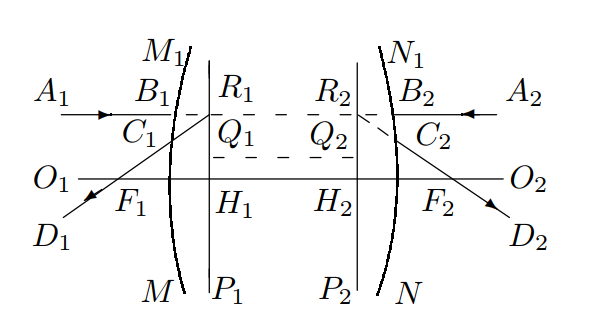
\includegraphics[width = 10cm]{1}}
	\caption{Ход лучей в толстой линзе}
	\label{fig:image}
\end{figure}

Рассмотрим теперь луч $A_2B_2$,
входящий в систему справа
и
лежащий на продолжении луча
$A_1B_1$. Слева из системы выйдет луч
$C_1D_1$, сопряжённый лучу $A_2B_2$. Точку
$F_1$ называют \textsl{передним фокусом системы} (фокусом
в пространстве предметов).
Исходящие из него лучи
в пространстве изображений параллельны
оптической оси. Продолжим
теперь $C_1D_1$ и $C_2D_2$ до пересечения с продолжениями
$A_1B_1$ и $A_2B_2$ и отметим точки пересечения $R_1$ и
$R_2$. Легко видеть, что эти точки
сопряжены, т.е. являются изображением друг друга. Действительно,
точка
$R_1$ лежит на пересечении лучей
$A_1B_1$ и
$C_1D_1$, а точка $R_2$ — на
пересечении сопряжённых им лучей
$A_2B_2$ и
$C_2D_2$ (для большей наглядности
направление одной пары сопряжённых лучей, например,
$A_2B_2$
и
$C_1D_1$, можно изменить на противоположное, пользуясь обратимостью
световых лучей). Из построения ясно, что точки
$R_1$ и
$R_2$ лежат на одинаковом
расстоянии от главной оптической оси, т.е.
$R_1H_1 = R_2H_2$ (поперечное
увеличение равно +1).


Можно показать, что в идеальной системе все точки плоскости
$P_1$,
перпендикулярной главной оптической оси
и проходящей через
$R_1$, попарно
сопряжены точкам плоскости
$P_2$, также перпендикулярной главной
оптической оси
и проходящей через
$R_2$. При этом сопряжённые точки
находятся на одинаковых расстояниях от оси (например, точки
$Q_1$ и $Q_2$). Плоскости
$P_1$ и
$P_2$ называются \textsl{главными плоскостями}, а точки $H_1$ и
$H_2$ — главными точками системы.
Расстояния от главных точек до фокусов называются фокусными
расстояниями: 
$f_1 = H_1F_1$, $f_2 = H_2F_2$. В том случае,
когда с обеих сторон системы находится одна и
та же среда (например, воздух),
$f_1 = f_2 = f$.


Если известно положение фокусов
и главных плоскостей, изображение
предмета может быть найдено путём простых геометрических построений.
Рисунок 2 иллюстрирует эти построения.


Удобно рассматривать лучи: а) падающие на линзу параллельно главной
оптической оси; б) проходящие через передний фокус линзы; в) проходящие
через центр линзы. Между главными плоскостями $P_1$ и $P_2$ все
лучи следует строить параллельно главной оптической оси. Для построения
изображения точки необходимо рассмотреть
ход двух любых лучей. Третий луч используют для проверки правильности построения изображения.

\begin{figure}[h!]
	\center{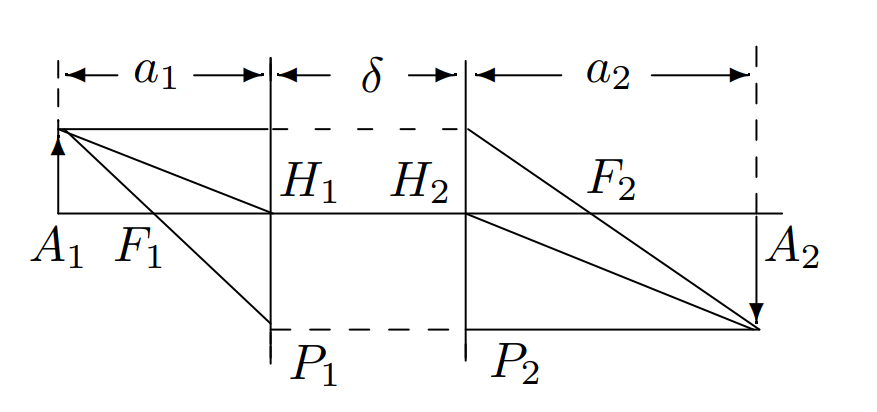
\includegraphics[width = 10cm]{2}}
	\caption{Построение изображения в толстой линзе}
	\label{fig:image}
\end{figure}

Оптическая система называется \textsl{положительной} или \textsl{собирающей},
если лучи, падающие на
неё параллельно главной оптической
оси, пройдя систему, отклоняются в направлении оси
— собираются.
Передний фокус $F_1$ в
этом случае лежит слева от главной
плоскости $P_1$, а задний фокус
$F_2$ — справа от
$P_2$. Если те
же лучи, пройдя систему, отклоняются от оси,
— система называется \textsl{отрицательной}, или \textsl{рассеивающей}. При этом с оптической осью пересекаются не сами лучи,
а их продолжения;
$F_1$ располагается правее $P_1$, а $F_2$ — левее $P_2$. Фокусному расстоянию приписывается определённый
знак: плюс для положительной системы и минус для отрицательной. Если
ввести расстояния от предмета и изображения до соответствующих главных плоскостей, то легко установить соотношение между этими расстояниями
и фокусным расстоянием системы:
\begin{equation}
\frac{1}{a_1} + \frac{1}{a_2} = \frac{1}{f}
\end{equation}

В формуле (1) $a_1$ считается положительным, если предмет лежит слева
от передней главной плоскости, $a_2$ положительно, если изображение
лежит справа от задней плоскости,
а фокусное расстояние
$f$ берётся со
своим знаком.
Следует подчеркнуть, что главные плоскости
и главные точки могут
лежать
как внутри, так
и вне системы
и при этом могут располагаться
асимметрично относительно поверхностей, ограничивающих оптическую
систему.
Большой практический интерес представляет случай,
когда размер
оптической системы в направлении главной оптической оси значительно
меньше фокусного расстояния. Оптический луч, проходя внутри такой
системы, мало смещается, поэтому главные плоскости
$P_1$ и
$P_2$ (рис. 2)
практически совпадают
и располагаются где-то посередине системы.
Такая
оптическая система называется тонкой линзой. Формула (1) остаётся,
конечно, справедливой
и для тонкой линзы; расстояния
$a_1$ и $a_2$ и фокусное расстояние
$f$ можно в этом случае приближённо отсчитывать
от центра линзы.

\vspace{1cm}
\textbf{I. Определение фокусного расстояния тонкой положительной линзы}

Фокусные расстояния тонких положительных линз можно определять
различными способами. Как было выяснено выше, в "приближении
тонкой линзы" считается, что обе главные плоскости совпадают и
проходят через середину линзы. Отсчитывая расстояния от середины
линзы до предмета
и до изображения, мы допускаем ошибку порядка
толщины стекла. При необходимости получить более точные значения
$f$
приходится отбросить «приближение тонкой линзы»
и учитывать расстояние
$\delta$ между главными плоскостями.

\begin{figure}[h!]
	\center{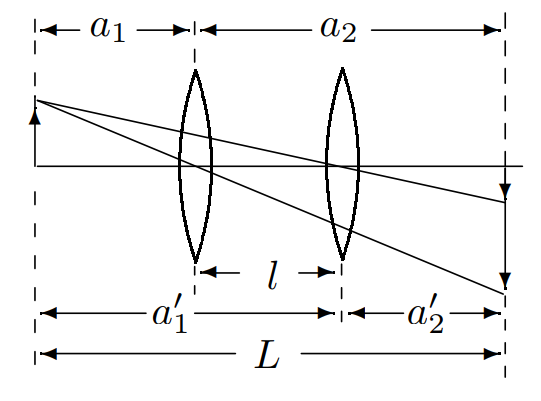
\includegraphics[width = 10cm]{3}}
	\caption{Измерение фокусного расстояния тонкой положительной линзы}
	\label{fig:image}
\end{figure}

\textsl{Способ 1.} Фокусное расстояние тонкой положительной линзы можно
определить, исходя из формулы линзы. Для этого достаточно измерить
расстояния $a_1$ и $a_2$ (рис. 2), полагая $\delta \rightarrow 0$, и затем вычислить
$f$ по формуле (1).
Проведя измерения при увеличенном
и при уменьшенном изображении
(рис. 3),
а также при различных положениях
предмета и изображения, можно
найти среднее значение фокусного расстояния.
Точность определения фокусного расстояния
по формуле линзы зависит от
расстояния между предметом
и изображением.


\textsl{Способ 2.} Пусть расстояние между предметом
и экраном превышает $4f$. Нетрудно убедиться, что при этом всегда найдутся два таких
положения линзы, при
которых на экране получаются отчётливые изображения
предмета (в одном случае уменьшенное, в другом
— увеличенное). Из соображений симметрии ясно, что
$a_1 = a_2'$ и $a_2 = a_1'$ (рис. 3).
Обозначая расстояние между предметом
и экраном через
$L$, а расстояние
между двумя поло
жениями линзы через $l$, получим:
$L = a_1 + a_2$; $l = a_1' − a_1 = a_2' − a_2$. Отсюда
\begin{equation}
a_1 = \frac{L-l}{2};~~a_2 = \frac{L+l}{2}
\end{equation}

Подставляя (2) в формулу линзы (1), найдём после несложных преобразований:
\begin{equation}
f = \frac{L^2 - l^2}{4L}
\end{equation}

Для определения фокусного расстояния достаточно, таким образом, измерить
расстояние
$L$ между предметом
и экраном
и расстояние $l$ между
двумя положениями линзы, при
которых на экране видны чёткие изображения.


\textsl{Способ 3.} Фокусное расстояние тонкой положительной линзы можно
определить с помощью зрительной трубы, настроенной на бесконечность,
то есть на параллельный пучок лучей.
Разместив между предметом
и зрительной трубой положительную
линзу
и перемещая её вдоль оси системы, можно найти резкое изображение
предмета в окуляре зрительной трубы. При этом расстояние от
середины линзы до предмет
а равно фокусному расстоянию тонкой линзы.
Для толстой линзы зрительная труба позволяет определить только
положение главного фокуса.

\vspace{1cm}
\textbf{II. Определение фокусного расстояния тонкой отрицательной линзы}

\textsl{Способ 1.} Определение фокусного расстояния отрицательной линзы
затруднено тем, что изображение предмета получается мнимым
(при действительном источнике)
и поэтому не может быть получено на
экране. Эту трудность легко обойти с помощью вспомогательной положительной
линзы.

\begin{figure}[h!]
	\center{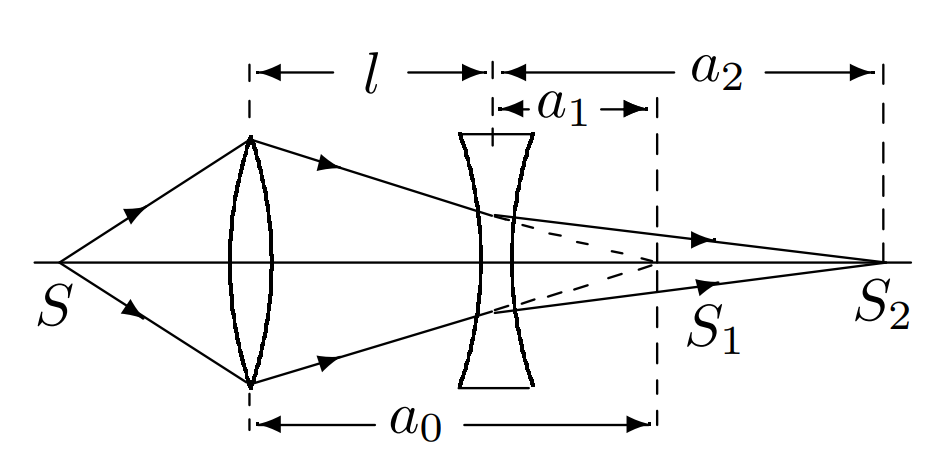
\includegraphics[width = 10cm]{4}}
	\caption{Измерение фокусного расстояния отрицательной линзы}
	\label{fig:image}
\end{figure}

Сначала с помощью положительной
линзы получают на экране
действительное изображение предмета
$S$ (точка $S_1$ на рис. 4). Затем
на пути лучей, выходящих из положительной
линзы, располагают исследуемую
отрицательную линзу и,
отодвигая экран, получают четкое
изображение предмета на экране,
образованное двумя линзами.
Точка
$S_1$ пересечения сходящихся лучей играет по отношению
к отрицательной
линзе роль мнимого источника. Изображение источник
а переместится теперь в точку $S_2$.


Определив расстояния $a_1$ $(a_1 = a_0 − l)$ и
$a_2$, рассчитывают фокусное
расстояние рассеивающей линзы по формуле (1).

\textsl{Способ 2.} Если расстояние
$a_1$ (рис. 4) совпадает с фокусным расстоянием
отрицательной линзы, то изображение перемещается в бесконечность,
т. е. лучи выходят из линзы параллельным пучком.
Параллельность пучка можно
установить с помощью зрительной трубы,
настроенной на бесконечность. Зная расстояние от первой линзы до
точки
$S_1$ и расстояние между линзами, нетрудно определить фокусное
расстояние тонкой отрицательной линзы. Для толстой отрицательной
линзы этот метод позволяет определить только положение главного фокуса.

\vspace{1cm}
\textbf{III. Определение фокусного расстояния и поло
жения главных плоскостей
сложной оптической системы}

Ни один из описанных выше способов не позволяет определить фокусное
расстояние
и положение главных плоскостей толстой линзы, т. е.
такой оптической системы, толщина
которой не мала по сравнению с
фокусным расстоянием.

\begin{figure}[h!]
	\center{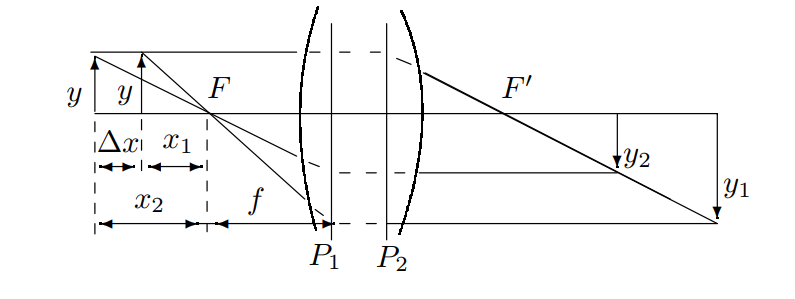
\includegraphics[width = 10cm]{5}}
	\caption{Измерения фокусного расстояния оптической системы по методу Аббе}
	\label{fig:image}
\end{figure}

Фокусное расстояние толстой положительной линзы определяют по
методу Аббе (рис. 5). Пусть предмет, линейный размер
которого равен
$y$,
находится на расстоянии
$x_1$ от главного фокуса
$F$ положительной оптической
системы. Изображение предмета имеет размер
$y_1$. Линейное
увеличение
$\beta_1$ равно
\begin{equation}
\beta_1 = \frac{y_1}{y} = \frac{f}{x_1}
\end{equation}

Если теперь отодвинуть предмет от линзы на расстояние $\Delta x$, то линейное
увеличение $\beta_2$ окажется равным
\begin{equation}
\beta_2 = \frac{y_2}{y} = \frac{f}{x_2}
\end{equation}

Из (4) и (5) нетрудно получить
\begin{equation}
f = \frac{\Delta x}{1/\beta_1 - 1/\beta_2}
\end{equation}

где $\Delta x = x_2 - x_1$ - — перемещение предмета.
Таким образом, для определения фокусного расстояния толстой положительной линзы нужно измерить
линейное увеличение системы при двух положениях предмета и
расстояние между этими двумя положениями.


Для нахождения главных плоскостей системы недостаточно знать
фокусное расстояние, нужно определить ещё положения главных фокусов.
Это можно сделать при помощи зрительной трубы, настроенной на бесконечность. Отложив от главных фокусов отрезки, равные фокусному
расстоянию, можно найти положения главных плоскостей системы.
Теоретически фокусное расстояние
$f'$ сложной системы, состоящей из
двух тонких положительных линз, можно рассчитать, если известны
фокусные расстояния
каждой линзы и расстояние между их центрами
$l_{12}$:
\begin{equation}
\frac{1}{f'} = \frac{1}{f_1'} + \frac{1}{f_2'} - \frac{|l_{12}|}{f_1'f_2'}
\end{equation}

\textbf{Экспериментальная
установка.} Оптическая скамья с осветителем,
набор линз, экран
и зрительная труба позволяют определить параметры
оптических систем всеми описанными способами. Все оптические элементы
устанавливаются на скамье при помощи рейтеров.

Важную роль играет правильная центрировка элементов системы.
Проходя через плохо отцентрированную систему, лучи свет
а могут отклониться
и пройти мимо экрана или глаза наблюдателя. Центрировать
линзы следует
как по высоте, так
и в поперечном направлении (для чего
линзы
установлены на поперечных салазках). 

\clearpage

\textbf{Ход работы}

Отцентрируем систему, не касаясь линз пальцами. После этого можно приступать к началу работы.

\textbf{Определение фокусных расстояний тонких линз при помощи экрана} 

Установим положительную линзу 1 между осветителем
и экраном.
Расположим экран на расстоянии
$L > 4f$ от предмета (рис. 3). Перемещая
линзу вдоль скамьи, получим увеличенное
и уменьшенное изображения предмета (края ирисовой диафрагмы) на экране.


\textbf{Метод Аббе}
С помощью линейки измерим расстояния от линзы до предмета
и до изображения ($a_1$, $a_2$, $a_1'$, $a_2'$ на рис. 3).

\begin{center}
\begin{tabular}{|c|c|c|c|c|c|c|c|c|c|c|c|c|c|}
\hline
$a_1$, см	&	$a_2$, см	&	$a_1'$, см	&	$a_2'$, см	&	$y_1$, см	&	$y_1'$, см	&	$y_2$, см	&	$y_2'$, см	\\
\hline
12.0		&	76.2		&	16.1		&	30.0		&	2.0			&	12.7		&	2.0			&	3.9			\\
\hline
\end{tabular}
\end{center}

Откуда
\begin{center}
\begin{tabular}{|c|c|c|c|c|c|c|c|c|c|c|c|}
\hline
$\Delta x$, см	&	$\Delta x'$, см	&	$\Delta(y'/y)$, см	&	$\Delta(y/y')$, см	\\
\hline
4.1				&	-46.2			&	0.39				&	4.44				\\
\hline
\end{tabular}
\end{center}

Отсюда по формуле (1):
$$
	f = \frac{\Delta x}{\Delta(y/y')} = -\frac{\Delta x'}{\Delta (y'/y)}
$$

Определим фокусное расстояние линзы:
$$
	f_1 = 10.4\text{см}
$$

Погрешность оценим, считая погрешность прямых измерений равной 1мм. Тогда:
$$
	f_1 = (10.4 \pm 0.9)\text{см}
$$

Аналогично для второй линзы:

\begin{center}
\begin{tabular}{|c|c|c|c|c|c|c|c|c|c|c|c|c|c|}
\hline
$a_1$, см	&	$a_2$, см	&	$a_1'$, см	&	$a_2'$, см	&	$y_1$, см	&	$y_1'$, см	&	$y_2$, см	&	$y_2'$, см	\\
\hline
17.5		&	46.3		&	22.5		&	29.8		&	2.0			&	5.3			&	2.0			&	2.7			\\
\hline
\end{tabular}
\end{center}

\begin{center}
\begin{tabular}{|c|c|c|c|c|c|c|c|c|c|c|c|}
\hline
$\Delta x$, см	&	$\Delta x'$, см	&	$\Delta(y'/y)$, см	&	$\Delta(y/y')$, см	\\
\hline
5.0				&	-16.5			&	0.39				&	1.29				\\
\hline
\end{tabular}
\end{center}

Откуда
$$
	f_2 = (12.8 \pm 0.9)\text{см}
$$

\textbf{Метод Бесселя}

Поставим экран и источник на расстоянии, превышающем учетверенное фокусное расстояние линзы. Найдем два положения, при которых мы наблюдаем четкое изображение, и найдем расстоние между положениями линзы. Независимо измерим расстояние $L$ от предмета до экрана
и перемещение линзы (рейтера) $l$. $l$ найдем как разность расстояний от источника до линзы.

По результатам измерений определим значение фокусного расстояния,
используя формулу (3).

\begin{center}
\begin{tabular}{|c|c|c|c|c|c|c|c|c|c|c|c|c|c|}
\hline
$L$, см		&	$a_1$, см	&	$a_1'$, см	&	$l$, см		\\
\hline
103.5		&	12.1		&	91.4		&	79.3		\\
\hline
\end{tabular}
\end{center}

Откуда, зная, что
$$
	f_1 = \frac{L^2 - l^2}{4L}
$$

$$
	f_1 = (10.5 \pm 0.1)\text{см}
$$

Аналогично для второй линзы:
\begin{center}
\begin{tabular}{|c|c|c|c|c|c|c|c|c|c|c|c|c|c|}
\hline
$L$, см		&	$a_1$, см	&	$a_1'$, см	&	$l$, см		\\
\hline
112.7		&	15.2		&	97.5		&	82.3		\\
\hline
\end{tabular}
\end{center}

$$
	f_2 = (13.1 \pm 0.1)\text{см}
$$

Для определения фокусного расстояния тонкой отрицательной линзы используем
вспомогательную положительную линзу. Сначала с помощью
короткофокусной положительной линзы получим на экране увеличенное
изображение предмета
и измерим линейкой расстояние от линзы до
экрана ($a_0$ на рис. 4). Затем между положительной линзой
и экраном
разместим рассеивающую линзу и, отодвигая экран от линзы, найдем
действительное изображение предмета, образованное системой линз. Измерим
расстояние
$a_2$ от рассеивающей линзы до экрана
и расстояние
между линзами $l$.
Рассчитаем величину $a_1$ и определим фокусное расстояние рассеивающей
линзы с помощью формулы (1).

\begin{center}
\begin{tabular}{|c|c|c|c|c|c|c|c|c|c|c|c|c|c|}
\hline
$a_0$, см	&	$l$, см		&	$a$, см		&	$a'$, см	\\
\hline
40.0		&	34.0		&	6.0			&	57.4		\\
\hline
\end{tabular}
\end{center}

Откуда:
$$
	f = \left(-\frac{1}{a} + \frac{1}{a'}\right) = (-6.7 \pm 0.4)\text{см}
$$


\vspace{1cm}
\textbf{Определение фокусных расстояний тонких линз с помощью
зрительной трубы}

Для определения фокусных расстояний линз с помощью зрительной трубы
необходимо настроить трубу на бесконечность. Эту настройку проще
всего осуществить, наведя трубу на
удалённый объект (например, на
окно в конце длинного
коридора).

Поставим положительную линзу на расстоянии от предмета примерно
равном фокусному. На небольшом расстоянии от линзы закрепим трубу,
настроенную на бесконечность,
и отцентрируем её по высоте. Передвигая
линзу вдоль скамьи, сначала получим в окуляре зрительной трубы
изображение поверхности матового стекла; затем, перемещая линзу с
помощью поперечных салазок
и меняя диаметр светового пятна с помощью
ирисовой диафрагмы, настроимся на чёткое изображение края
диафрагмы. При этом расстояние между предметом
и серединой тонкой
линзы (между проточками на оправах) равно фокусному.

Повернем линзу другой стороной к источнику и повторим измерения фокусного расстояния. Аналогично измерим фокусное расстояние второй линзы.

Получим:
\begin{center}
\begin{tabular}{|c|c|c|c|c|c|c|c|c|c|c|c|c|}
\hline
$f_{1_1}$, см	&	$f_{1_2}$, см	&	$f_{2_1}$, см	&	$f_{2_2}$, см	\\
\hline
10.5			&	10.0			&	12.8			&	12.7			\\
\hline
\end{tabular}
\end{center}

Для определения фокусного расстояния тонкой отрицательной линзы используем
схему, изображённую на рис. 4. Сначала получим на экране
увеличенное изображение диафрагмы при помощи
короткофокусной положительной
линзы. Измерим расстояние
$a_0$ между линзой и экраном.

Разместим сразу за экраном трубу, настроенную на бесконечность,
и закрепим её. Уберем экран и поставим на его место исследуемую
рассеивающую линзу. Отцентрируем световой пучок с помощью листа
бумаги. Перемещая рассеивающую линзу, найдем в окуляре зрительной
трубы резкое изображение края диафрагмы.
Подберем оптимальную яркость источника.
Измерив расстояние между линзами $l$, рассчитаем фокусное расстояние
рассеивающей линзы:
$f' = a_0 − l$.

Повернем рассеивающую линзу другой стороной
к источнику
и повторим
измерения.

\begin{center}
\begin{tabular}{|c|c|c|c|c|c|c|c|c|c|c|c|c|}
\hline
$a_0$, см	&	$l_1$, см	&	$f_1$, см	&	$l_2$, см	&	$f_2$, см	\\
\hline
32.5		&	25.7		&	6.8			&	25.5		&	7.0			\\
\hline
\end{tabular}
\end{center}


\vspace{1cm}
\textbf{Определение фокусного расстояния сложной оптической системы}

Для создания сложной оптической системы
установим в центре оптической
скамьи две тонких собирающих линзы на расстоянии, в полтора-два
раза превышающем сумму их фокусов,
и закрепим рейтеры. Измерим расстояние $l_{12}$ между линзами.

Для определения фокусного расстояния системы по формуле (6) расположим
экран на дальнем конце скамьи.
Установим на осветителе диафрагму диаметром 1 см (по риске на
оправе осветителя) и, перемещая осветитель вдоль скамьи, получим
на экране резкое изображение диафрагмы. Измерим расстояние от диафрагмы
до первой линзы и величину изображения $y_1$ (см. рис. 5).
Отодвинем источник на несколько сантиметров от прежнего положения
и, передвигая экран, вновь получим резкое изображение диафрагмы.
Для повышения точности размеры изображений
$y_1$ и
$y_2$ должны
заметно отличаться друг от друга. Измерив расстояние от предмета до
первой линзы
и рассчитав перемещение
$\Delta x$, определим фокусное расстояние
системы по формуле (6).

\begin{center}
\begin{tabular}{|c|c|c|c|c|c|c|c|c|c|c|c|c|c|}
\hline
$a_1$, см	&	$b_1$, см	&	$a_2$, см	&	$b_2$, см	&	$l$, см		\\
\hline
4.7			&	66.7		&	9.3			&	15.5		&	8.4			\\
\hline
\end{tabular}
\end{center}

Отсюда
\begin{center}
\begin{tabular}{|c|c|c|c|c|c|c|c|c|c|c|c|}
\hline
$\Delta x$, см	&	$\Delta x'$, см	&	$\Delta(y'/y)$, см	&	$\Delta(y/y')$, см	\\
\hline
4.6				&	-51.2			&	0.51				&	5.68				\\
\hline
\end{tabular}
\end{center}

Отсюда найдем $f$ двумя способами:
$$
	f_{\text{Аббе}} = (9.2 \pm 0.7)\text{см}
$$
$$
	f_2 = (9.0 \pm 0.5)\text{см}
$$

Для нахождения положения главных фокусов системы закрепим зрительную
трубу за второй линзой, подвинем осветитель
к первой линзе и отцентрируем систему с помощью листа бумаги.
Медленно отодвигая осветитель от системы, сначала найдем резкое
изображение поверхности стекла в окуляре зрительной трубы,
а затем,
последовательно уменьшая размер пятна
и перемещая пятно с помощью
винта поперечных салазок линзы, настроимся на край ирисовой диафрагмы.
Определим положение переднего главного
фокуса системы, измерив расстояние $\Delta$ от предмета до первой линзы.

Отсюда:
$$
	f_{front} = 9.0\text{см}
$$

Развернем систему и повторим измерения. Получим:
$$
	f_{back} = 9.4\text{см}
$$

\vspace{1cm}
\textbf{Сферическая абберация} 

Снимем зависимоть смещения $\Delta s$ от радиуса диафрагмы $h$:
\begin{center}
\begin{tabular}{|c|c|c|c|c|c|c|c|c|c|c|}
\hline
$h$, см	&	$\Delta s$, см	&	$h^2$, см$^2$	\\
\hline
0.5		&	0				&	0.3				\\
\hline
1.0		&	-1.0			&	1.0				\\
\hline
2.0		&	-2.5			&	4.0				\\
\hline
\end{tabular}
\end{center}

\vspace{1cm}
\begin{tikzpicture}
\begin{axis}[
	height = 10cm,
	width  = 15cm,
	every axis y label/.style={at = {(ticklabel cs: 0.5)}, rotate = 90, anchor = near ticklabel},
	xlabel = {$h^2$, см},
	ylabel = {$\Delta s$, см},
	grid   = major
]
\addplot+[
	only marks,
	error bars/.cd, 
	y dir = both, y explicit,
	x dir = both, x explicit,
	]
coordinates{
	(0.3, 0) +- (0.1, 0.1)
	(1.0, -1) +- (0.1, 0.1)
	(4.0, -2.5) +- (0.3, 0.1)
};

\addplot [mark = none]
coordinates{
	(0.3, -0.252373)
	(4, -2.55889)
};

\end{axis}
\end{tikzpicture}

Зная, что
$$
	\Delta s(h) = \frac{R}{n-1}\left(1 - \frac{n^2h^2}{2R^2}\right)
$$
	
Нетрудно получить:
$$
	n = 1.6 \pm 0.2
$$

\clearpage

Таким образом, в данной лабораторной работе мы изучили поведение оптических систем и области применимости законов, подразумевающих "тонкость" линзы.

\end{document}